% Cover, title page and copyright page of the PDF edition.
\thispagestyle{empty}
\AddToShipoutPictureBG*{\AtPageLowerLeft{%
  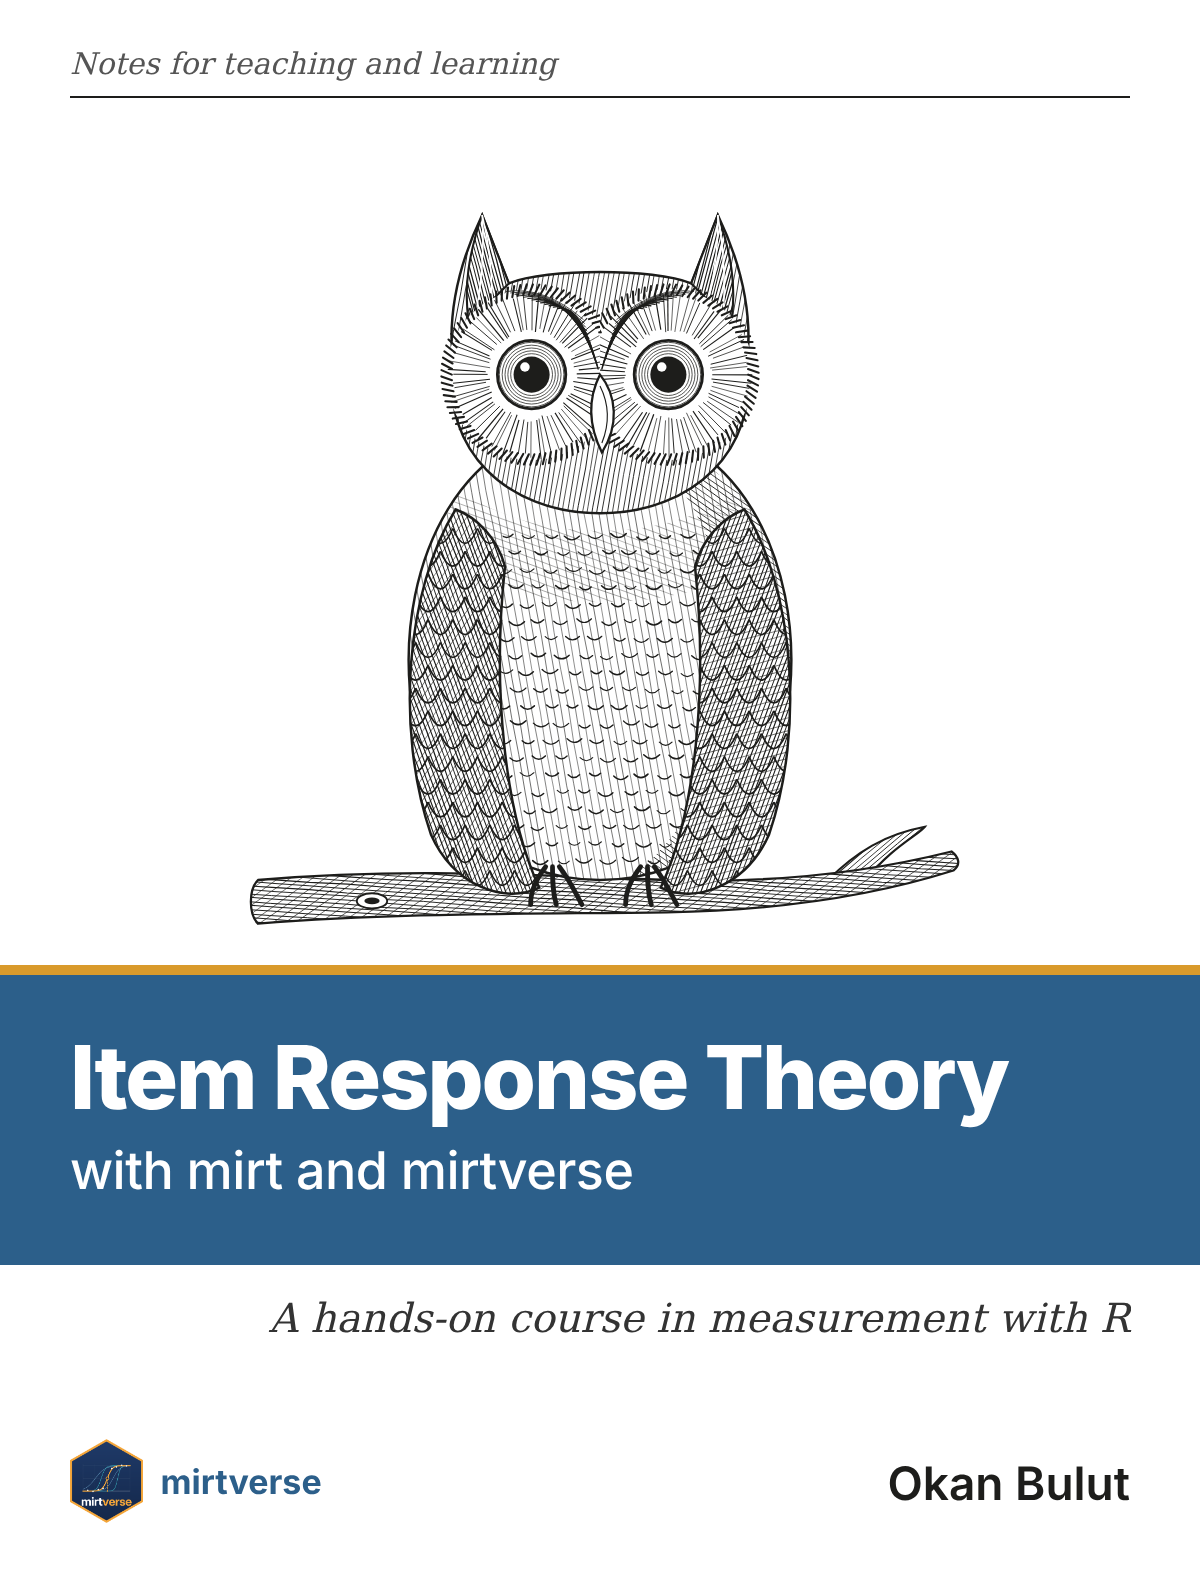
\includegraphics[width = \paperwidth, height = \paperheight]{cover/cover.png}}}
\mbox{}
\cleardoublepage

\begin{titlepage}
\centering
\vspace*{3cm}
{\sffamily\bfseries\fontsize{30}{36}\selectfont\color{mvdark} Item Response Theory\par}
\vspace{0.4em}
{\sffamily\LARGE\color{mvnavy} with mirt and mirtverse\par}
\vspace{1.2em}
{\color{mvamber}\rule{0.35\textwidth}{1.5pt}\par}
\vspace{1.2em}
{\Large\itshape Notes for teaching and learning\par}
\vfill
{\sffamily\bfseries\Large Okan Bulut\par}
\vspace{0.6em}
{\large Measurement, Evaluation, and Data Science\\ University of Alberta\par}
\vspace{0.8em}
\href{mailto:bulut@ualberta.ca}{bulut@ualberta.ca}\quad\textperiodcentered\quad
\href{http://www.okanbulut.com}{www.okanbulut.com}\par
\vspace{2.5cm}
\end{titlepage}

\thispagestyle{empty}
\vspace*{\fill}
\begin{flushleft}\small
\textit{Item Response Theory with mirt and mirtverse: Notes for Teaching and
Learning}\\
by Okan Bulut

\bigskip
\textcopyright{} \the\year{} Okan Bulut. The text and figures of this book
are licensed under a Creative Commons Attribution-NonCommercial-ShareAlike
4.0 International licence
(\href{https://creativecommons.org/licenses/by-nc-sa/4.0/}{CC BY-NC-SA 4.0}).
The R code is licensed under GPL-3.

\bigskip
DOI: \href{https://doi.org/10.5281/zenodo.23885605}{10.5281/zenodo.23885605}\\
Online edition: \url{https://www.okanbulut.com/mirtverse/book/}\\
Source: \url{https://github.com/okanbulut/mirtverse/tree/main/book}

\bigskip
Typeset with bookdown and XeLaTeX on \today. The cover illustration is an
original engraving-style drawing made for this book.
\end{flushleft}
\clearpage
